\documentclass[12pt]{article}
\usepackage{hyperref,setspace,graphicx,fancyhdr}
\usepackage[]{accessibility}
\usepackage[width=6in,height=9in]{geometry}
% changes font to TeX Gyre Schola (Century Schoolbook)
\usepackage{tgschola}\usepackage[T1]{fontenc}

\newcounter{authornote}[page]
\newcommand{\authornote}[1]{\renewcommand{\thefootnote}{\fnsymbol{footnote}}\stepcounter{authornote}\footnote[\value{authornote}]{#1}\renewcommand{\thefootnote}{\arabic{footnote}}}

\newcommand{\hbreak}{\par\noindent\begin{tabular*}{\linewidth}{c}\hline\hline\end{tabular*}\par}

\newcommand*{\authortitle}[1]{\centerline{\Huge\sc #1}}

\begin{document}
\authortitle{C.S. Peirce}

\bigskip

\paragraph{About Peirce:}
Charles Sanders Peirce (1839--1914) was born in Cambridge,
Massachusetts. (His last name rhymes with \emph{purse}, not with \emph{fierce}.) His father, Benjamin Peirce. was Professor of Mathematics at
Harvard University, one of the founders of the U.S. Coast and
Geodetic Survey, and one of the founders of the Smithsonian
Institution.

Peirce graduated from Harvard in 1859. He was then
employed by the U.S. Coast and Geodetic Survey, mainly surveying and
carrying out geodetic investigations. From 1879 through 1884, Peirce
also taught logic in the Department of Mathematics at Johns Hopkins University. This job ended suddenly for reasons that
apparently connected to Peirce cohabiting with his wife before marriage. Peirce's position with the the Coast and Geodetic Survey was
terminated in late 1891 because of a congressional funding decision. For the remainder of his life, Peirce eked out a living doing odd-jobs and consulting work--- mainly in chemical engineering and analysis. Peirce was often in dire financial straits; at times he managed to survive only through the charity of friends, including his old college chum William James.

Peirce's writings extend from about 1857 to near his
death, his published works run to about 12,000 printed pages, and his known unpublished manuscripts run to about 80,000 handwritten pages. The topics on which he wrote have an immense range: mathematics, logic, metaphysics, physical science, economics, the theory of signs\ldots

\paragraph{About this text:}
This document is prepared by \href{https://www.fecundity.com}{P.D. Magnus} from various sources. The biography is adapted from Robert Burch's contribution to the \href{http://plato.stanford.edu}{\emph{Stanford Encyclopedia of Philosophy}}.

% This file does not have the appropriate header and tags to compile in latex. It is meant to be input into another file for compiling. 
% This document is based on electronic transcriptions by Joseph Ransdell and Brian Kariger, which used to be available at the Arisbe website: http://www.iupui.edu/~arisbe/

\section*{[from] Some Consequences of Four Incapacities Claimed For Man}
\emph{This paper was originally published in the \emph{Journal of Speculative Philosophy} 2 (1868), pgs. 140--157. These opening paragraphs reveal Peirce's pragmatic temperament.}

Descartes is the father of modern philosophy, and the spirit of Cartesianism--- that which principally distinguishes it from the scholasticism which it displaced--- may be compendiously stated as follows:

1. It teaches that philosophy must begin with universal doubt; whereas scholasticism had never questioned fundamentals.

2. It teaches that the ultimate test of certainty is to be found in the individual consciousness; whereas scholasticism had rested on the testimony of sages and of the Catholic Church.

3. The multiform argumentation of the middle ages is replaced by a single thread of inference depending often upon inconspicuous premisses.

4. Scholasticism had its mysteries of faith, but undertook to explain all created things. But there are many facts which Cartesianism not only does not explain but renders absolutely inexplicable, unless to say that ``God makes them so'' is to be regarded as an explanation.

In some, or all of these respects, most modern philosophers have been, in effect, Cartesians. Now without wishing to return to scholasticism, it seems to me that modern science and modern logic require us to stand upon a very different platform from this.

1. We cannot begin with complete doubt. We must begin with all the prejudices which we actually have when we enter upon the study of philosophy. These prejudices are not to be dispelled by a maxim, for they are things which it does not occur to us \emph{can} be questioned. Hence this initial skepticism will be a mere self-deception, and not real doubt; and no one who follows the Cartesian method will ever be satisfied until he has formally recovered all those beliefs which in form he has given up. It is, therefore, as useless a preliminary as going to the North Pole would be in order to get to Constantinople by coming down regularly upon a meridian. A person may, it is true, in the course of his studies, find reason to doubt what he began by believing; but in that case he doubts because he has a positive reason for it, and not on account of the Cartesian maxim. Let us not pretend to doubt in philosophy what we do not doubt in our hearts.

2. The same formalism appears in the Cartesian criterion, which amounts to this: ``Whatever I am clearly convinced of, is true.'' If I were really convinced, I should have done with reasoning and should require no test of certainty. But thus to make single individuals absolute judges of truth is most pernicious. The result is that metaphysicians will all agree that metaphysics has reached a pitch of certainty far beyond that of the physical sciences; --- only they can agree upon nothing else. In sciences in which men come to agreement, when a theory has been broached it is considered to be on probation until this agreement is reached. After it is reached, the question of certainty becomes an idle one, because there is no one left who doubts it. We individually cannot reasonably hope to attain the ultimate philosophy which we pursue; we can only seek it, therefore, for the \emph{community} of philosophers. Hence, if disciplined and candid minds carefully examine a theory and refuse to accept it, this ought to create doubts in the mind of the author of the theory himself.

3. Philosophy ought to imitate the successful sciences in its methods, so far as to proceed only from tangible premisses which can be subjected to careful scrutiny, and to trust rather to the multitude and variety of its arguments than to the conclusiveness of any one. Its reasoning should not form a chain which is no stronger than its weakest link, but a cable whose fibers may be ever so slender, provided they are sufficiently numerous and intimately connected.

4. Every unidealistic philosophy supposes some absolutely inexplicable, unanalyzable ultimate; in short, something resulting from mediation itself not susceptible of mediation. Now that anything is thus inexplicable can only be known by reasoning from signs. But the only justification of an inference from signs is that the conclusion explains the fact. To suppose the fact absolutely inexplicable, is not to explain it, and hence this supposition is never allowable.

\ldots

% This file does not have the appropriate header and tags to compile in latex. It is meant to be input into another file for compiling. 
% This document is based on electronic transcriptions by Joseph Ransdell and Brian Kariger, which used to be available at the Arisbe website: http://www.iupui.edu/~arisbe/

\section*{The Fixation of Belief}
\emph{This paper was published in \emph{Popular Science Monthly} 12 (November 1877), pgs. 1--15. It is the first in a series of six essays, together titled ``Illustrations of the Logic of Science.'' A further essay was planned, and the collection was once listed as a forthcoming book in Appleton's International Scientific Series.}

\subsection*{I}


Few persons care to study logic, because everybody conceives himself to be proficient enough in the art of reasoning already. But I observe that this satisfaction is limited to one's own ratiocination, and does not extend to that of other men.

We come to the full possession of our power of drawing inferences the last of all our faculties, for it is not so much a natural gift as a long and difficult art. The history of its practice would make a grand subject for a book. The medieval schoolmen, following the Romans, made logic the earliest of a boy's studies after grammar, as being very easy. So it was, as they understood it. Its fundamental principle, according to them, was, that all knowledge rests on either authority or reason; but that whatever is deduced by reason depends ultimately on a premise derived from authority. Accordingly, as soon as a boy was perfect in the syllogistic procedure, his intellectual kit of tools was held to be complete.

To Roger Bacon, that remarkable mind who in the middle of the thirteenth century was almost a scientific man, the schoolmen's conception of reasoning appeared only an obstacle to truth. He saw that experience alone teaches any\-thing--- a proposition which to us seems easy to understand, because a distinct conception of experience has been handed down to us from former generations; which to him also seemed perfectly clear, because its difficulties had not yet unfolded themselves. Of all kinds of experience, the best, he thought, was interior illumination, which teaches many things about Nature which the external senses could never discover, such as the transubstantiation of bread.

Four centuries later, the more celebrated Bacon, in the first book of his \emph{Novum Organum}, gave his clear account of experience as something which must be open to verification and re-examination. But, superior as Lord Bacon's conception is to earlier notions, a modern reader who is not in awe of his grandiloquence is chiefly struck by the inadequacy of his view of scientific procedure. That we have only to make some crude experiments, to draw up briefs of the results in certain blank forms, to go through these by rule, checking off everything disproved and setting down the alternatives, and that thus in a few years physical science would be finished up--- what an idea! ``He wrote on science like a Lord Chancellor,'' indeed. 

The early scientists, Copernicus, Tycho Brahe, Kepler, Galileo, and Gilbert, had methods more like those of their modern brethren. Kepler undertook to draw a curve through the places of Mars;\authornote{Not quite so, but as nearly so as can be told in a few words.} and his greatest service to science was in impressing on men's minds that this was the thing to be done if they wished to improve astronomy; that they were not to content themselves with inquiring whether one system of epicycles was better than another, but that they were to sit down to the figures and find out what the curve, in truth, was. He accomplished this by his incomparable energy and courage, blundering along in the most inconceivable way (to us), from one irrational hypothesis to another, until, after trying twenty-two of these, he fell, by the mere exhaustion of his invention, upon the orbit which a mind well furnished with the weapons of modern logic would have tried almost at the outset.

In the same way, every work of science great enough to be well remembered for a few generations affords some exemplification of the defective state of the art of reasoning of the time when it was written; and each chief step in science has been a lesson in logic. It was so when Lavoisier and his contemporaries took up the study of chemistry. The old chemist's maxim had been, ``\emph{Lege, lege, lege, labora, ora, et relege}.'' [In Latin: ``Read, read, read, work, pray, and read again.''] Lavoisier's method was not to read and pray, not to dream that some long and complicated chemical process would have a certain effect, [but] to put it into practice with dull patience, after its inevitable failure, to dream that with some modification it would have another result, and to end by publishing the last dream as a fact: his way was to carry his mind into his laboratory, and to make of his alembics and cucurbits instruments of thought, giving a new conception of reasoning as something which was to be done with one's eyes open, by manipulating real things instead of words and fancies.

The Darwinian controversy is, in large part, a question of logic. Mr. Darwin proposed to apply the statistical method to biology. The same thing had been done in a widely different branch of science, the theory of gases. Though unable to say what the movements of any particular molecule of gas would be on a certain hypothesis regarding the constitution of this class of bodies, Clausius and Maxwell were yet able, by the application of the doctrine of probabilities, to predict that in the long run such and such a proportion of the molecules would, under given circumstances, acquire such and such velocities; that there would take place, every second, such and such a number of collisions, etc.; and from these propositions were able to deduce certain properties of gases, especially in regard to their heat-relations. In like manner, Darwin, while unable to say what the operation of variation and natural selection in any individual case will be, demonstrates that in the long run they will adapt animals to their circumstances. Whether or not existing animal forms are due to such action, or what position the theory ought to take, forms the subject of a discussion in which questions of fact and questions of logic are curiously interlaced.

\subsection*{II}

The object of reasoning is to find out, from the consideration of what we already know, something else which we do not know. Consequently, reasoning is good if it be such as to give a true conclusion from true premises, and not otherwise. Thus, the question of its validity is purely one of fact and not of thinking. A being the premises and B the conclusion, the question is, whether these facts are really so related that if A is B is. If so, the inference is valid; if not, not. It is not in the least the question whether, when the premisses are accepted by the mind, we feel an impulse to accept the conclusion also. It is true that we do generally reason correctly by nature. But that is an accident; the true conclusion would remain true if we had no impulse to accept it; and the false one would remain false, though we could not resist the tendency to believe in it.

We are, doubtless, in the main logical animals, but we are not perfectly so. Most of us, for example, are naturally more sanguine and hopeful than logic would justify. We seem to be so constituted that in the absence of any facts to go upon we are happy and self-satisfied; so that the effect of experience is continually to contract our hopes and aspirations. Yet a lifetime of the application of this corrective does not usually eradicate our sanguine disposition. Where hope is unchecked by any experience, it is likely that our optimism is extravagant. Logicality in regard to practical matters is the most useful quality an animal can possess, and might, therefore, result from the action of natural selection; but outside of these it is probably of more advantage to the animal to have his mind filled with pleasing and encouraging visions, independently of their truth; and thus, upon unpractical subjects, natural selection might occasion a fallacious tendency of thought.


That which determines us, from given premises, to draw one inference rather than another, is some habit of mind, whether it be constitutional or acquired. The habit is good or otherwise, according as it produces true conclusions from true premisses or not; and an inference is regarded as valid or not, without reference to the truth or falsity of its conclusion specially, but according as the habit which determines it is such as to produce true conclusions in general or not. The particular habit of mind which governs this or that inference may be formulated in a proposition whose truth depends on the validity of the inferences which the habit determines; and such a formula is called a \emph{guiding principle} of inference. Suppose, for example, that we observe that a rotating disk of copper quickly comes to rest when placed between the poles of a magnet, and we infer that this will happen with every disk of copper. The guiding principle is, that what is true of one piece of copper is true of another. Such a guiding principle with regard to copper would be much safer than with regard to many other substances--- brass, for example.


A book might be written to signalize all the most important of these guiding principles of reasoning. It would probably be, we must confess, of no service to a person whose thought is directed wholly to practical subjects, and whose activity moves along thoroughly-beaten paths. The problems which present themselves to such a mind are matters of routine which he has learned once for all to handle in learning his business. But let a man venture into an unfamiliar field, or where his results are not continually checked by experience, and all history shows that the most masculine intellect will ofttimes lose his orientation and waste his efforts in directions which bring him no nearer to his goal, or even carry him entirely astray. He is like a ship in the open sea, with no one on board who understands the rules of navigation. And in such a case some general study of the guiding principles of reasoning would be sure to be found useful.

The subject could hardly be treated, however, without being first limited; since almost any fact may serve as a guiding principle. But it so happens that there exists a division among facts, such that in one class are all those which are absolutely essential as guiding principles, while in the others are all which have any other interest as objects of research. This division is between those which are necessarily taken for granted in asking whether a certain conclusion follows from certain premises, and those which are not implied in that question. A moment's thought will show that a variety of facts are already assumed when the logical question is first asked. It is implied, for instance, that there are such states of mind as doubt and belief--- that a passage from one to the other is possible, the object of thought remaining the same, and that this transition is subject to some rules which all minds are alike bound by. As these are facts which we must already know before we can have any clear conception of reasoning at all, it cannot be supposed to be any longer of much interest to inquire into their truth or falsity. On the other hand, it is easy to believe that those rules of reasoning which are deduced from the very idea of the process are the ones which are the most essential; and, indeed, that so long as it conforms to these it will, at least, not lead to false conclusions from true premisses. In point of fact, the importance of what may be deduced from the assumptions involved in the logical question turns out to be greater than might be supposed, and this for reasons which it is difficult to exhibit at the outset. The only one which I shall here mention is, that conceptions which are really products of logical reflection, without being readily seen to be so, mingle with our ordinary thoughts, and are frequently the causes of great confusion. This is the case, for example, with the conception of quality. A quality, as such, is never an object of observation. We can see that a thing is blue or green, but the quality of being blue and the quality of being green are not things which we see; they are products of logical reflections. The truth is, that common-sense, or thought as it first emerges above the level of the narrowly practical, is deeply imbued with that bad logical quality to which the epithet \emph{metaphysical} is commonly applied; and nothing can clear it up but a severe course of logic.

\subsection*{III}

We generally know when we wish to ask a question and when we wish to pronounce a judgment, for there is a dissimilarity between the sensation of doubting and that of believing.

But this is not all which distinguishes doubt from belief. There is a practical difference. Our beliefs guide our desires and shape our actions. The Assassins, or followers of the Old Man of the Mountain, used to rush into death at his least command, because they believed that obedience to him would insure everlasting felicity. Had they doubted this, they would not have acted as they did. So it is with every belief, according to its degree. The feeling of believing is a more or less sure indication of there being established in our nature some habit which will determine our actions. Doubt never has such an effect.

Nor must we overlook a third point of difference. Doubt is an uneasy and dissatisfied state from which we struggle to free ourselves and pass into the state of belief; while the latter is a calm and satisfactory state which we do not wish to avoid, or to change to a belief in anything else.\authornote{ I am not speaking of secondary effects occasionally produced by the interference of other impulses.} On the contrary, we cling tenaciously, not merely to believing, but to believing just what we do believe.


Thus, both doubt and belief have positive effects upon us, though very different ones. Belief does not make us act at once, but puts us into such a condition that we shall behave in some certain way, when the occasion arises. Doubt has not the least effect of this sort, but stimulates us to action until it is destroyed. This reminds us of the irritation of a nerve and the reflex action produced thereby; while for the analogue of belief, in the nervous system, we must look to what are called nervous associations--- for example, to that habit of the nerves in consequence of which the smell of a peach will make the mouth water.

\subsection*{IV}

The irritation of doubt causes a struggle to attain a state of belief. I shall term this struggle \emph{inquiry}, though it must be admitted that this is sometimes not a very apt designation.


The irritation of doubt is the only immediate motive for the struggle to attain belief. It is certainly best for us that our beliefs should be such as may truly guide our actions so as to satisfy our desires; and this reflection will make us reject any belief which does not seem to have been so formed as to insure this result. But it will only do so by creating a doubt in the place of that belief. With the doubt, therefore, the struggle begins, and with the cessation of doubt it ends. Hence, the sole object of inquiry is the settlement of opinion. We may fancy that this is not enough for us, and that we seek, not merely an opinion, but a true opinion. But put this fancy to the test, and it proves groundless; for as soon as a firm belief is reached we are entirely satisfied, whether the belief be true or false. And it is clear that nothing out of the sphere of our knowledge can be our object, for nothing which does not affect the mind can be the motive for mental effort. The most that can be maintained is, that we seek for a belief that we shall \emph{think}  to be true. But we think each one of our beliefs to be true, and, indeed, it is mere tautology to say so.

That the settlement of opinion is the sole end of inquiry is a very important proposition. It sweeps away, at once, various vague and erroneous conceptions of proof. A few of these may be noticed here.

1. Some philosophers have imagined that to start an inquiry it was only necessary to utter a question or set in down upon paper, and have even recommended us to begin our studies with questioning everything!  But the mere putting of a proposition into the interrogative form does not stimulate the mind to any struggle after belief.  There must be a real and living doubt, and without this all discussion is idle. 

2. It is a very common idea that a demonstration must rest on some ultimate and absolutely indubitable propositions. These, according to one school, are first principles of a general nature; according to another, are first sensations. But, in point of fact, an inquiry, to have that completely satisfactory result called demonstration, has only to start with propositions perfectly free from all actual doubt. If the premisses are not in fact doubted at all, they cannot be more satisfactory than they are.

3. Some people seem to love to argue a point after all the world is fully convinced of it. But no further advance can be made. When doubt ceases, mental action on the subject comes to an end; and, if it did go on, it would be without a purpose.

\subsection*{V}

If the settlement of opinion is the sole object of inquiry, and if belief is of the nature of a habit, why should we not attain the desired end, by taking any answer to a question which we may fancy, and constantly reiterating it to ourselves, dwelling on all which may conduce to that belief, and learning to turn with contempt and hatred from anything that might disturb it? This simple and direct method is really pursued by many men. I remember once being entreated not to read a certain newspaper lest it might change my opinion upon free-trade. ``Lest I might be entrapped by its fallacies and misstatements,'' was the form of expression. ``You are not,'' my friend said, ``a special student of political economy. You might, therefore, easily be deceived by fallacious arguments upon the subject. You might, then, if you read this paper, be led to believe in protection. But you admit that free-trade is the true doctrine; and you do not wish to believe what is not true.'' I have often known this system to be deliberately adopted. Still oftener, the instinctive dislike of an undecided state of mind, exaggerated into a vague dread of doubt, makes men cling spasmodically to the views they already take. The man feels that, if he only holds to his belief without wavering, it will be entirely satisfactory. Nor can it be denied that a steady and immovable faith yields great peace of mind. It may, indeed, give rise to inconveniences, as if a man should resolutely continue to believe that fire would not burn him, or that he would be eternally damned if he received his \emph{ingesta} otherwise than through a stomach-pump. But then the man who adopts this method will not allow that its inconveniences are greater than its advantages. He will say, ``I hold steadfastly to the truth, and the truth is always wholesome.'' And in many cases it may very well be that the pleasure he derives from his calm faith overbalances any inconveniences resulting from its deceptive character. Thus, if it be true that death is annihilation, then the man who believes that he will certainly go straight to heaven when he dies, provided he have fulfilled certain simple observances in this life, has a cheap pleasure which will not be followed by the least disappointment. A similar consideration seems to have weight with many persons in religious topics, for we frequently hear it said, ``Oh, I could not believe so-and-so, because I should be wretched if I did.'' When an ostrich buries its head in the sand as danger approaches, it very likely takes the happiest course. It hides the danger, and then calmly says there is no danger; and, if it feels perfectly sure there is none, why should it raise its head to see? A man may go through life, systematically keeping out of view all that might cause a change in his opinions, and if he only succeeds--- basing his method, as he does, on two fundamental psychological laws--- I do not see what can be said against his doing so. It would be an egotistical impertinence to object that his procedure is irrational, for that only amounts to saying that his method of settling belief is not ours. He does not propose to himself to be rational, and, indeed, will often talk with scorn of man's weak and illusive reason. So let him think as he pleases.

But this method of fixing belief, which may be called the method of tenacity, will be unable to hold its ground in practice. The social impulse is against it. The man who adopts it will find that other men think differently from him, and it will be apt to occur to him, in some saner moment, that their opinions are quite as good as his own, and this will shake his confidence in his belief. This conception, that another man's thought or sentiment may be equivalent to one's own, is a distinctly new step, and a highly important one. It arises from an impulse too strong in man to be suppressed, without danger of destroying the human species. Unless we make ourselves hermits, we shall necessarily influence each other's opinions; so that the problem becomes how to fix belief, not in the individual merely, but in the community.

Let the will of the state act, then, instead of that of the individual. Let an institution be created which shall have for its object to keep correct doctrines before the attention of the people, to reiterate them perpetually, and to teach them to the young; having at the same time power to prevent contrary doctrines from being taught, advocated, or expressed. Let all possible causes of a change of mind be removed from men's apprehensions. Let them be kept ignorant, lest they should learn of some reason to think otherwise than they do. Let their passions be enlisted, so that they may regard private and unusual opinions with hatred and horror. Then, let all men who reject the established belief be terrified into silence. Let the people turn out and tar-and-feather such men, or let inquisitions be made into the manner of thinking of suspected persons, and when they are found guilty of forbidden beliefs, let them be subjected to some signal punishment. When complete agreement could not otherwise be reached, a general massacre of all who have not thought in a certain way has proved a very effective means of settling opinion in a country. If the power to do this be wanting, let a list of opinions be drawn up, to which no man of the least independence of thought can assent, and let the faithful be required to accept all these propositions, in order to segregate them as radically as possible from the influence of the rest of the world.

This method has, from the earliest times, been one of the chief means of upholding correct theological and political doctrines, and of preserving their universal or catholic character. In Rome, especially, it has been practised from the days of Numa Pompilius to those of Pius Nonus. This is the most perfect example in history; but wherever there is a priesthood--- and no religion has been without one--- this method has been more or less made use of. Wherever there is an aristocracy, or a guild, or any association of a class of men whose interests depend, or are supposed to depend, on certain propositions, there will be inevitably found some traces of this natural product of social feeling. Cruelties always accompany this system; and when it is consistently carried out, they become atrocities of the most horrible kind in the eyes of any rational man. Nor should this occasion surprise, for the officer of a society does not feel justified in surrendering the interests of that society for the sake of mercy, as he might his own private interests. It is natural, therefore, that sympathy and fellowship should thus produce a most ruthless power.

In judging this method of fixing belief, which may be called the method of authority, we must, in the first place, allow its immeasurable mental and moral superiority to the method of tenacity. Its success is proportionately greater; and, in fact, it has over and over again worked the most majestic results. The mere structures of stone which it has caused to be put together--- in Siam, for example, in Egypt, and in Europe--- have many of them a sublimity hardly more than rivaled by the greatest works of Nature. And, except the geological epochs, there are no periods of time so vast as those which are measured by some of these organized faiths. If we scrutinize the matter closely, we shall find that there has not been one of their creeds which has remained always the same; yet the change is so slow as to be imperceptible during one person's life, so that individual belief remains sensibly fixed. For the mass of mankind, then, there is perhaps no better method than this. If it is their highest impulse to be intellectual slaves, then slaves they ought to remain.

But no institution can undertake to regulate opinions upon every subject. Only the most important ones can be attended to, and on the rest men's minds must be left to the action of natural causes. This imperfection will be no source of weakness so long as men are in such a state of culture that one opinion does not influence another--- that is, so long as they cannot put two and two together. But in the most priest-ridden states some individuals will be found who are raised above that condition. These men possess a wider sort of social feeling; they see that men in other countries and in other ages have held to very different doctrines from those which they themselves have been brought up to believe; and they cannot help seeing that it is the mere accident of their having been taught as they have, and of their having been surrounded with the manners and associations they have, that has caused them to believe as they do and not far differently. And their candor cannot resist the reflection that there is no reason to rate their own views at a higher value than those of other nations and other centuries; and this gives rise to doubts in their minds.

They will further perceive that such doubts as these must exist in their minds with reference to every belief which seems to be determined by the caprice either of themselves or of those who originated the popular opinions. The willful adherence to a belief, and the arbitrary forcing of it upon others, must, therefore, both be given up, and a new method of settling opinions must be adopted, which shall not only produce an impulse to believe, but shall also decide what proposition it is which is to be believed. Let the action of natural preferences be unimpeded, then, and under their influence let men, conversing together and regarding matters in different lights, gradually develop beliefs in harmony with natural causes. This method resembles that by which conceptions of art have been brought to maturity. The most perfect example of it is to be found in the history of metaphysical philosophy. Systems of this sort have not usually rested upon any observed facts, at least not in any great degree. They have been chiefly adopted because their fundamental propositions seemed ``agreeable to reason.'' This is an apt expression; it does not mean that which agrees with experience, but that which we find ourselves inclined to believe. Plato, for example, finds it agreeable to reason that the distances of the celestial spheres from one another should be proportional to the different lengths of strings which produce harmonious chords. Many philosophers have been led to their main conclusions by considerations like this; but this is the lowest and least developed form which the method takes, for it is clear that another man might find Kepler's theory, that the celestial spheres are proportional to the inscribed and circumscribed spheres of the different regular solids, more agreeable to \emph{his} reason. But the shock of opinions will soon lead men to rest on preferences of a far more universal nature. Take, for example, the doctrine that man only acts selfishly--- that is, from the consideration that acting in one way will afford him more pleasure than acting in another. This rests on no fact in the world, but it has had a wide acceptance as being the only reasonable theory.

This method is far more intellectual and respectable from the point of view of reason than either of the others which we have noticed. But its failure has been the most manifest. It makes of inquiry something similar to the development of taste; but taste, unfortunately, is always more or less a matter of fashion, and accordingly metaphysicians have never come to any fixed agreement, but the pendulum has swung backward and forward between a more material and a more spiritual philosophy, from the earliest times to the latest. And so from this, which has been called the \emph{a priori} method, we are driven, in Lord Bacon's phrase, to a true induction. We have examined into this \emph{a priori} method as something which promised to deliver our opinions from their accidental and capricious element. But development, while it is a process which eliminates the effect of some casual circumstances, only magnifies that of others. This method, therefore, does not differ in a very essential way from that of authority. The government may not have lifted its finger to influence my convictions; I may have been left outwardly quite free to choose, we will say, between monogamy and polygamy, and, appealing to my conscience only, I may have concluded that the latter practice is in itself licentious. But when I come to see that the chief obstacle to the spread of Christianity among a people of as high culture as the Hindoos has been a conviction of the immorality of our way of treating women, I cannot help seeing that, though governments do not interfere, sentiments in their development will be very greatly determined by accidental causes. Now, there are some people, among whom I must suppose that my reader is to be found, who, when they see that any belief of theirs is determined by any circumstance extraneous to the facts, will from that moment not merely admit in words that that belief is doubtful, but will experience a real doubt of it, so that it ceases to be a belief.


To satisfy our doubts, therefore, it is necessary that a method should be found by which our beliefs may be caused by nothing human, but by some external permanency--- by something upon which our thinking has no effect. Some mystics imagine that they have such a method in a private inspiration from on high. But that is only a form of the method of tenacity, in which the conception of truth as something public is not yet developed. Our external permanency would not be external, in our sense, if it was restricted in its influence to one individual. It must be something which affects, or might affect, every man. And, though these affections are necessarily as various as are individual conditions, yet the method must be such that the ultimate conclusion of every man shall be the same. Such is the method of science. Its fundamental hypothesis, restated in more familiar language, is this: There are real things, whose characters are entirely independent of our opinions about them; those realities affect our senses according to regular laws, and, though our sensations are as different as are our relations to the objects, yet, by taking advantage of the laws of perception, we can ascertain by reasoning how things really are; and any man, if he have sufficient experience and reason enough about it, will be led to the one true conclusion. The new conception here involved is that of reality. It may be asked how I know that there are any realities. If this hypothesis is the sole support of my method of inquiry, my method of inquiry must not be used to support my hypothesis. The reply is this: 1. If investigation cannot be regarded as proving that there are real things, it at least does not lead to a contrary conclusion; but the method and the conception on which it is based remain ever in harmony. No doubts of the method, therefore, necessarily arise from its practice, as is the case with all the others. 2. The feeling which gives rise to any method of fixing belief is a dissatisfaction at two repugnant propositions. But here already is a vague concession that there is some \emph{one} thing to which a proposition should conform.  Nobody, therefore, can really doubt that there are realities, or, if he did, doubt would not be a source of dissatisfaction. The hypothesis, therefore, is one which every mind admits. So that the social impulse does not cause me to doubt it. 3. Everybody uses the scientific method about a great many things, and only ceases to use it when he does not know how to apply it. 4. Experience of the method has not led me to doubt it, but, on the contrary, scientific investigation has had the most wonderful triumphs in the way of settling opinion. These afford the explanation of my not doubting the method or the hypothesis which it supposes; and not having any doubt, nor believing that anybody else whom I could influence has, it would be the merest babble for me to say more about it. If there be anybody with a living doubt upon the subject, let him consider it.


To describe the method of scientific investigation is the object of this series of papers. At present I have only room to notice some points of contrast between it and other methods of fixing belief.

This is the only one of the four methods which presents any distinction of a right and a wrong way. If I adopt the method of tenacity, and shut myself out from all influences, whatever I think necessary to doing this is necessary according to that method. So with the method of authority: the state may try to put down heresy by means which, from a scientific point of view, seem very ill-calculated to accomplish its purposes; but the only test \emph{on that method} is what the state thinks; so that it cannot pursue the method wrongly. So with the \emph{a priori} method. The very essence of it is to think as one is inclined to think. All metaphysicians will be sure to do that, however they may be inclined to judge each other to be perversely wrong. The Hegelian system recognizes every natural tendency of thought as logical, although it be certain to be abolished by counter-tendencies. Hegel thinks there is a regular system in the succession of these tendencies, in consequence of which, after drifting one way and the other for a long time, opinion will at last go right. And it is true that metaphysicians do get the right ideas at last; Hegel's system of Nature represents tolerably the science of that day; and one may be sure that whatever scientific investigation has put out of doubt will presently receive \emph{a priori} demonstration on the part of the metaphysicians. But with the scientific method the case is different. I may start with known and observed facts to proceed to the unknown; and yet the rules which I follow in doing so may not be such as investigation would approve. The test of whether I am truly following the method is not an immediate appeal to my feelings and purposes, but, on the contrary, itself involves the application of the method. Hence it is that bad reasoning as well as good reasoning is possible; and this fact is the foundation of the practical side of logic.

It is not to be supposed that the first three methods of settling opinion present no advantage whatever over the scientific method. On the contrary, each has some peculiar convenience of its own. The \emph{a priori} method is distinguished for its comfortable conclusions. It is the nature of the process to adopt whatever belief we are inclined to, and there are certain flatteries to the vanity of man which we all believe by nature, until we are awakened from our pleasing dream by some rough facts. The method of authority will always govern the mass of mankind; and those who wield the various forms of organized force in the state will never be convinced that dangerous reasoning ought not to be suppressed in some way. If liberty of speech is to be untrammeled from the grosser forms of constraint, then uniformity of opinion will be secured by a moral terrorism to which the respectability of society will give its thorough approval. Following the method of authority is the path of peace. Certain non-conformities are permitted; certain others (considered unsafe) are forbidden. These are different in different countries and in different ages; but, wherever you are, let it be known that you seriously hold a tabooed belief, and you may be perfectly sure of being treated with a cruelty less brutal but more refined than hunting you like a wolf. Thus, the greatest intellectual benefactors of mankind have never dared, and dare not now, to utter the whole of their thought; and thus a shade of \emph{prima facie} doubt is cast upon every proposition which is considered essential to the security of society. Singularly enough, the persecution does not all come from without; but a man torments himself and is oftentimes most distressed at finding himself believing propositions which he has been brought up to regard with aversion. The peaceful and sympathetic man will, therefore, find it hard to resist the temptation to submit his opinions to authority. But most of all I admire the method of tenacity for its strength, simplicity, and directness. Men who pursue it are distinguished for their decision of character, which becomes very easy with such a mental rule. They do not waste time in trying to make up their minds what they want, but, fastening like lightning upon whatever alternative comes first, they hold to it to the end, whatever happens, without an instant's irresolution. This is one of the splendid qualities which generally accompany brilliant, unlasting success. It is impossible not to envy the man who can dismiss reason, although we know how it must turn out at last.

Such are the advantages which the other methods of settling opinion have over scientific investigation. A man should consider well of them; and then he should consider that, after all, he wishes his opinions to coincide with the fact, and that there is no reason why the results of those three first methods should do so. To bring about this effect is the prerogative of the method of science. Upon such considerations he has to make his choice--- a choice which is far more than the adoption of any intellectual opinion, which is one of the ruling decisions of his life, to which, when once made, he is bound to adhere. The force of habit will sometimes cause a man to hold on to old beliefs, after he is in a condition to see that they have no sound basis. But reflection upon the state of the case will overcome these habits, and he ought to allow reflection its full weight. People sometimes shrink from doing this, having an idea that beliefs are wholesome which they cannot help feeling rest on nothing. But let such persons suppose an analogous though different case from their own. Let them ask themselves what they would say to a reformed Mussulman who should hesitate to give up his old notions in regard to the relations of the sexes; or to a reformed Catholic who should still shrink from reading the Bible. Would they not say that these persons ought to consider the matter fully, and clearly understand the new doctrine, and then ought to embrace it, in its entirety? But, above all, let it be considered that what is more wholesome than any particular belief is integrity of belief, and that to avoid looking into the support of any belief from a fear that it may turn out rotten is quite as immoral as it is disadvantageous. The person who confesses that there is such a thing as truth, which is distinguished from falsehood simply by this, that if acted on it will carry us to the point we aim at and not astray, and then, though convinced of this, dares not know the truth and seeks to avoid it, is in a sorry state of mind indeed.

Yes, the other methods do have their merits: a clear logical conscience does cost something--- just as any virtue, just as all that we cherish, costs us dear. But we should not desire it to be otherwise.  The genius of a man's logical method should be loved and reverenced as his bride, whom he has chosen from all the world.  He need not condemn the others; on the contrary, he may honor them deeply, and in doing so he only honors her the more.  But she is the one that he has chosen, and he knows that he was right in making that choice.  And having made it, he will work and fight for her, and will not complain that there are blows to take, hoping that there may be as many and as hard to give, and will strive to be the worthy knight and champion of her from the blaze of whose splendors he draws his inspiration and his courage.


% This file does not have the appropriate header and tags to compile in latex. It is meant to be input into another file for compiling. 
% This document is based on electronic transcriptions by Joseph Ransdell and Brian Kariger, which used to be available at the Arisbe website: http://www.iupui.edu/~arisbe/

\section*{How to Make Our Ideas Clear}
\emph{This is the sequel to ``The Fixation of Belief'' and can be read as a continuation of the same argument. It was originally published in \emph{Popular Science Monthly} 12 (January 1878), pgs. 286--302.}

\subsection*{I}

Whoever has looked into a modern treatise on logic of the common sort, will doubtless remember the two distinctions between \emph{clear} and \emph{obscure} conceptions, and between \emph{distinct} and \emph{confused} conceptions. They have lain in the books now for nigh two centuries, unimproved and unmodified, and are generally reckoned by logicians as among the gems of their doctrine.


A clear idea is defined as one which is so apprehended that it will be recognized wherever it is met with, and so that no other will be mistaken for it. If it fails of this clearness, it is said to be obscure.


This is rather a neat bit of philosophical terminology; yet, since it is clearness that they were defining, I wish the logicians had made their definition a little more plain. Never to fail to recognize an idea, and under no circumstances to mistake another for it, let it come in how recondite a form it may, would indeed imply such prodigious force and clearness of intellect as is seldom met with in this world. On the other hand, merely to have such an acquaintance with the idea as to have become familiar with it, and to have lost all hesitancy in recognizing it in ordinary cases, hardly seems to deserve the name of clearness of apprehension, since after all it only amounts to a subjective feeling of mastery which may be entirely mistaken. I take it, however, that when the logicians speak of ``clearness,'' they mean nothing more than such a familiarity with an idea, since they regard the quality as but a small merit, which needs to be supplemented by another, which they call \emph{distinctness.}

A distinct idea is defined as one which contains nothing which is not clear. This is technical language; by the \emph{contents} of an idea logicians understand whatever is contained in its definition. So that an idea is \emph{distinctly} apprehended, according to them, when we can give a precise definition of it, in abstract terms. Here the professional logicians leave the subject; and I would not have troubled the reader with what they have to say, if it were not such a striking example of how they have been slumbering through ages of intellectual activity, listlessly disregarding the enginery of modern thought, and never dreaming of applying its lessons to the improvement of logic. It is easy to show that the doctrine that familiar use and abstract distinctness make the perfection of apprehension has its only true place in philosophies which have long been extinct; and it is now time to formulate the method of attaining to a more perfect clearness of thought, such as we see and admire in the thinkers of our own time.

When Descartes set about the reconstruction of philosophy, his first step was to (theoretically) permit scepticism and to discard the practice of the schoolmen of looking to authority as the ultimate source of truth. That done, he sought a more natural fountain of true  principles, and thought he found it in the human mind; thus passing, in the directest way, from the method of authority to that of apriority, as described in my first paper. Self-consciousness was to furnish us with our fundamental truths, and to decide what was agreeable to reason. But since, evidently, not all ideas are true, he was led to note, as the first condition of infallibility, that they must be clear. The distinction between an idea \emph{seeming} clear and really being so, never occurred to him.  Trusting to introspection, as he did, even for a knowledge of external things, why should he question its testimony in respect to the contents of our own minds? But then, I suppose, seeing men, who seemed to be quite clear and positive, holding opposite opinions upon fundamental principles, he was further led to say that clearness of ideas is not sufficient, but that they need also to be distinct, i.e., to have nothing unclear about them. What he probably meant by this (for he did not explain himself with precision) was, that they must sustain the test of dialectical examination; that they must not only seem clear at the outset, but that discussion must never be able to bring to light points of obscurity connected with them.


Such was the distinction of Descartes, and one sees that it was precisely on the level of his philosophy. It was somewhat developed by Leibnitz. This great and singular genius was as remarkable for what he failed to see as for what he saw. That a piece of mechanism could not do work perpetually without being fed with power in some form, was a thing perfectly apparent to him; yet he did not understand that the machinery of the mind can only transform knowledge, but never originate it, unless it be fed with facts of observation. He thus missed the most essential point of the Cartesian philosophy, which is, that to accept propositions which seem perfectly evident to us is a thing which, whether it be logical or illogical, we cannot help doing. Instead of regarding the matter in this way, he sought to reduce the first principles of science to two classes, those which cannot be denied without self-contradiction, and those which result from the principle of sufficient reason (of which more anon), and was apparently unaware of the great difference between his position and that of Descartes. So he reverted to the old trivialities of logic; and, above all, abstract definitions played a great part in his philosophy. It was quite natural, therefore, that on observing that the method of Descartes labored under the difficulty that we may seem to ourselves to have clear apprehensions of ideas which in truth are very hazy, no better remedy occurred to him than to require an abstract definition of every important term. Accordingly, in adopting the distinction of \emph{clear} and \emph{distinct} notions, he described the latter quality as the clear apprehension of everything contained in the definition; and the books have ever since copied his words. There is no danger that his chimerical scheme will ever again be over-valued. Nothing new can ever be learned by analyzing definitions. Nevertheless, our existing  beliefs can be set in order by this process, and order is an essential element of intellectual economy, as of every other. It may be acknowledged, therefore, that the books are right in making familiarity with a notion the first step toward clearness of apprehension, and the defining of it the second. But in omitting all mention of any higher perspicuity of thought, they simply mirror a philosophy which was exploded a hundred years ago. That much-admired ``ornament of logic''--- the doctrine of clearness and distinctness--- may be pretty enough, but it is high time to relegate to our cabinet of curiosities the antique \emph{bijou,} and to wear about us something better adapted to modern uses.

The very first lesson that we have a right to demand that logic shall teach us is, how to make our ideas clear; and a most important one it is, depreciated only by minds who stand in need of it. To know what we think, to be masters of our own meaning, will make a solid foundation for great and weighty thought. It is most easily learned by those whose ideas are meagre and restricted; and far happier they than such as wallow helplessly in a rich mud of conceptions. A nation, it is true, may, in the course of generations, overcome the disadvantage of an excessive wealth of language and its natural concomitant, a vast, unfathomable deep of ideas. We may see it in history, slowly perfecting its literary forms, sloughing at length its metaphysics, and, by virtue of the untirable patience which is often a compensation, attaining great excellence in every branch of mental acquirement. The page of history is not yet unrolled that is to tell us whether such a people will or will not in the long run prevail over one whose ideas (like the words of their language) are few, but which  possesses a wonderful mastery over those which it has. For an individual, however, there can be no question that a few clear ideas are worth more than many confused ones. A young man would hardly be persuaded to sacrifice the greater part of his thoughts to save the rest; and the muddled head is the least apt to see the necessity of such a sacrifice. Him we can usually only commiserate, as a person with a congenital defect. Time will help him, but intellectual maturity with regard to clearness comes rather late, an unfortunate arrangement of Nature, inasmuch as clearness is of less use to a man settled in life, whose  errors have in great measure had their effect, than it would be to one whose path lay before him. It is terrible to see how a single unclear idea, a single formula without meaning, lurking in a young man's head, will sometimes act like an obstruction of inert matter in an artery, hindering the nutrition of the brain, and condemning its victim to pine away in the fullness of his intellectual vigor and in the midst of intellectual plenty. Many a man has cherished for years as his hobby some vague shadow of an idea, too meaningless to be positively false; he has, nevertheless, passionately loved it, has made it his companion by day and by night, and has given to it his strength and his life, leaving all other occupations for its sake, and in short has lived with it and for it, until it has become, as it were, flesh of his flesh and bone of his bone; and then he has waked up some bright morning to find it gone, clean vanished away like the beautiful Melusina of the fable, and the essence of his life gone with it. I have myself known such a man; and who can tell how many histories of circle-squarers, metaphysicians, astrologers, and what not, may not be told in the old German story?

\subsection*{II}

The principles set forth in the first part of these papers lead, at once, to a method of reaching a clearness of thought of a far higher grade than the ``distinctness'' of the logicians. We have there found that the action of thought is excited by the irritation of doubt, and ceases when belief is attained; so that the production of belief is the sole function of thought. All these words, however, are too strong for my purpose. It is as if I had described the phenomena as they appear under a mental microscope. Doubt and Belief, as the words are commonly employed, relate to religious or other grave discussions. But here I use them to designate the starting of any question, no matter how small or how great, and the resolution of it. If, for instance, in a horse-car, I pull out my purse and find a five-cent nickel and five coppers, I decide, while my hand is going to the purse, in which way I will pay my fare. To call such a question Doubt, and my decision Belief, is certainly to use words very disproportionate to the occasion. To speak of such a doubt as causing an irritation which needs to be appeased, suggests a temper which is uncomfortable to the verge of insanity. Yet, looking at the matter
minutely, it must be admitted that, if there is the least hesitation as to whether I shall pay the five coppers or the nickel (as there will be sure to be, unless I act  from some previously contracted habit in the matter), though irritation is too strong a word, yet I am excited to such small mental activity as may be necessary to deciding how I shall act. Most frequently doubts arise from some indecision, however momentary, in our action. Sometimes it is not so. I have, for example, to wait in a railway-station, and to pass the time I read the advertisements on the walls. I compare the advantages of different trains and different routes which I never expect to take, merely fancying myself to be in a state of hesitancy, because I am bored with having nothing to trouble me. Feigned hesitancy, whether feigned for mere amusement or with a lofty purpose, plays a great part in the production of scientific inquiry. However the doubt may originate, it stimulates the mind to an activity which may be slight or energetic, calm or turbulent. Images pass rapidly through consciousness, one incessantly melting into another, until at last, when all is over--- it may be in a fraction of a second, in an hour, or after long years--- we find ourselves decided as to how we should act under
such circumstances as those which occasioned our hesitation. In other words, we have attained belief.
 

In this process we observe two sorts of elements of consciousness, the distinction between which may best be made clear by means of an illustration. In a piece of music there are the separate notes, and there is the air. A single tone may be prolonged for an hour or a day, and it exists as perfectly in each second of that time as in the whole taken together; so that, as long as it is sounding, it might be present to a sense from which everything in the past was as completely absent as the future itself. But it is different with the air, the performance of which occupies a certain time, during the portions of which only portions of it are played. It consists in an orderliness in the succession of sounds which strike the ear at different times; and to perceive it there must be some continuity of consciousness which makes the events of a lapse of time present to us. We certainly only perceive the air by hearing the separate notes; yet we cannot be said to directly hear it, for we hear only what is present at the instant, and an orderliness of succession cannot exist in an instant. These two sorts of objects, what we are \emph{immediately} conscious of and what we are
\emph{mediately} conscious of, are found in all consciousness. Some elements (the sensations) are completely present at every instant so long as they last, while others (like thought) are actions having beginning, middle, and end, and consist in a congruence in the succession of sensations which flow through the  mind. They cannot be immediately present to us, but must cover some portion of the past or future. Thought is a thread of melody running through the succession of our sensations.


We may add that just as a piece of music may be written in parts, each part having its own air, so various systems of relationship of succession subsist together between the same sensations. These different systems are distinguished by having different motives, ideas, or functions. Thought is only one such system, for its sole motive, idea, and function is to produce belief, and whatever does not concern that purpose belongs to some other system of relations. The action of thinking may incidentally have other results; it may serve to amuse us, for example, and among \emph{dilettanti} it is not rare to find those who have so perverted thought to the purposes of pleasure that it seems to vex them to think that the questions upon which they delight to exercise it may ever get finally settled; and a positive discovery which takes a favorite subject out of the arena of literary debate is met with ill-concealed dislike. This disposition is the very debauchery of thought. But the soul and meaning of thought, abstracted from the other elements which accompany it, though it may be voluntarily thwarted, can never be made to direct itself toward anything but the production of belief. Thought in action has for its only possible motive the attainment of thought at rest; and whatever does not refer to belief is no part of the thought itself. 

And what, then, is belief? It is the demi-cadence which closes a musical phrase in the symphony of our intellectual life. We have seen that it has just three properties: First, it is something that we are aware of; second, it appeases the irritation of doubt; and, third, it involves the establishment in our nature of a rule of action, or, say for short, a \emph{habit.} As it appeases the irritation of doubt, which is the motive for thinking, thought relaxes, and comes to rest for a moment when belief is reached. But, since belief is a rule for action, the application of which involves further doubt and further thought, at the same time that it is a stopping-place, it is also a new starting-place for thought. That is why I have permitted myself to call it thought at rest, although thought is essentially an action. The \emph{final} upshot of thinking is the exercise of volition, and of this thought no longer forms a part; but belief is only a stadium of mental action, an effect upon our nature due to thought, which will influence future thinking.
 

The essence of belief is the establishment of a habit; and different  beliefs are distinguished by the different modes of action to which they give rise. If beliefs do not differ in this respect, if they appease the same doubt by producing the same rule of action, then no mere differences in the manner of consciousness of them can make them different beliefs, any more than playing a tune in different keys is playing different tunes. Imaginary distinctions are often drawn between beliefs which differ only in their mode of expression; --- the wrangling which ensues is real enough, however. To believe that any objects are arranged among themselves as in Fig. 1, and to believe that they are arranged in Fig. 2 are one and the same belief;

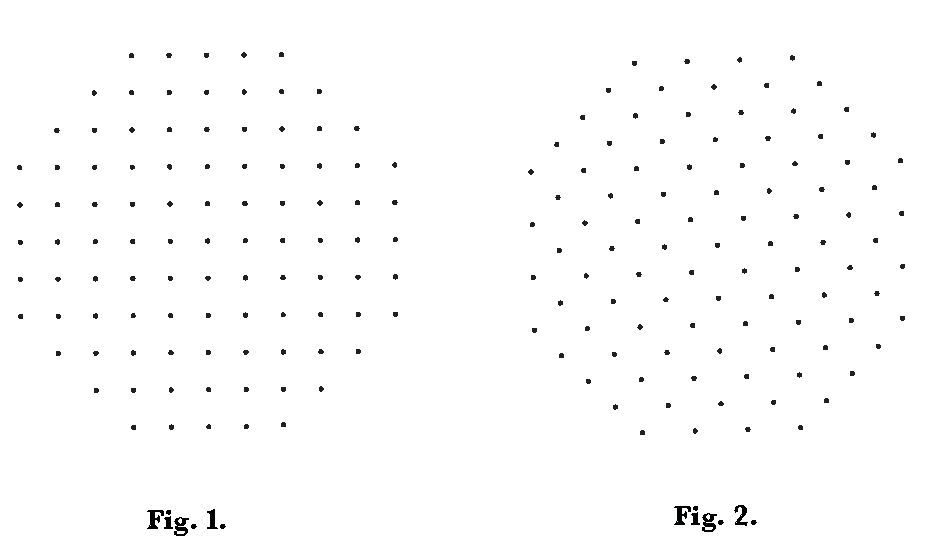
\includegraphics[width=3.6in]{peirce-howto1.pdf}

yet it is conceivable that a man should assert one proposition and deny the other. Such false distinctions do as much harm as the confusion of beliefs really different, and are among the pitfalls of which we ought constantly to beware, especially when we are upon metaphysical ground. One singular deception of this sort, which often occurs, is to mistake the sensation produced by our own unclearness of thought for a character of the object we are thinking. Instead of perceiving that the obscurity is purely subjective, we fancy that we contemplate a quality of the object which is essentially mysterious; and if our conception be afterward presented to us in a clear form we do not recognize it as the same, owing to the absence of the feeling of unintelligibility. So long as this deception lasts, it obviously puts an impassable barrier in the way of perspicuous thinking; so that it equally interests the opponents of rational thought to perpetuate it, and its adherents to guard against it.


Another such deception is to mistake a mere difference in the grammatical construction of two words for a distinction between the ideas they express. In this pedantic age, when the general mob of writers attend so much more to words than to things, this error is common enough. When I just said that thought is an \emph{action,} and that it consists in a \emph{relation,} although a person performs an action but not a relation, which can only be the result of an action, yet there was no inconsistency in what I said, but only a grammatical vagueness. 

From all these sophisms we shall be perfectly safe so long as we reflect that the whole function of thought is to produce habits of action; and that whatever there is connected with a thought, but irrelevant to its purpose, is an accretion to it, but no part of it. If there be a unity among our sensations which has no reference to how we shall act on a given occasion, as when we listen to a piece of music, why we do not call that thinking. To develop its meaning, we have, therefore, simply to determine what habits it produces, for what a thing means is simply what habits it involves. Now, the identity of a habit depends on how it might lead us to act, not merely under such circumstances as are likely to arise, but under such as might possibly occur, no matter how improbable they may be. What the habit is depends on \emph{when} and \emph{how} it causes us to act. As for the \emph{when,} every stimulus to action is derived from perception; as for the \emph{how,} every purpose of action is to produce some sensible result. Thus, we come down to what is tangible and conceivably practical, as the root of every real distinction of thought, no matter how subtile it may be; and there is no distinction of meaning so fine as to consist in anything but a possible difference of practice.


To see what this principle leads to, consider in the light of it such a doctrine as that of transubstantiation. The Protestant churches generally hold that the elements of the sacrament are flesh and blood only in a tropical sense; they nourish our souls as meat and the juice of it would our bodies. But the Catholics maintain that they are literally just meat and blood; although they possess all the sensible qualities of wafercakes and diluted wine. But we can have no conception of wine except what may enter into a belief, either ---
\begin{quote}
1. That this, that, or the other, is wine; or,\\
2. That wine possesses certain properties.
\end{quote}

Such beliefs are nothing but self-notifications that we should, upon occasion, act in regard to such things as we believe to be wine according to the qualities which we believe wine to possess. The occasion  of such action would be some sensible perception, the motive of it to produce some sensible result. Thus our action has exclusive reference to what affects the senses, our habit has the same bearing as our action, our belief the same as our habit, our conception the same as our belief; and we can consequently mean nothing by wine but what has certain effects, direct or indirect, upon our senses; and to talk of something as having all the sensible characters of wine, yet being in reality blood, is senseless jargon. Now, it is not my object to pursue the theological question; and having used it as a logical example I drop it, without caring to anticipate the theologian's reply. I only desire to point out how impossible it is that we should have an idea in our minds which relates to anything but conceived sensible effects of things. Our idea of anything \emph{is} our idea of its sensible effects; and if we fancy that we have any other we deceive ourselves, and mistake a mere sensation accompanying the thought for a part of the thought itself. It is absurd to say that thought has any meaning unrelated to its only function. It is foolish for Catholics and Protestants to fancy themselves in disagreement about the elements of the sacrament, if they agree in regard to all their sensible effects, here and hereafter.
It appears, then, that the rule for attaining the third grade of clearness of apprehension is as follows: Consider what effects, which might conceivably have practical bearings, we conceive the object of our conception to have. Then, our conception of these effects is the whole of our conception of the object.


\subsection*{III}

Let us illustrate this rule by some examples; and, to begin with the simplest one possible, let us ask what we mean by calling a thing \emph{hard}. Evidently that it will not be scratched by many other substances. The whole conception of this quality, as of every other, lies in its conceived effects. There is absolutely no difference between a hard thing and a soft thing so long as they are not brought to the test. Suppose, then, that a diamond could be crystallized in the midst of a cushion of soft cotton, and should remain there until it was finally burned up. Would it be false to say that that diamond was soft? This seems a foolish question, and would be so, in fact, except in the realm of logic. There such questions are often of the greatest utility as serving to bring logical principles into sharper relief than real discussions ever could. In studying logic we must not put them aside with hasty answers, but must consider them with attentive care, in order  to make out the principles involved. We may, in the present case, modify our question, and ask what prevents us from saying that all hard bodies remain perfectly soft until they are touched, when their hardness increases with the pressure until they are scratched. Reflection will show that the reply is this: there would be no \emph{falsity} in such modes of speech. They would involve a modification of our present usage of speech with regard to the words hard and soft, but not of their meanings. For they represent no fact to be different from what it is; only they involve arrangements of facts which would be exceedingly maladroit. This leads us to remark that the question of what would occur under circumstances which do not actually arise is not a question of fact, but only of the most perspicuous arrangement of them. For example, the question of free-will and fate in its simplest form, stripped of verbiage, is something like this: I have done something of which I am ashamed; could I, by an effort of the will, have resisted the temptation, and done otherwise? The philosophical reply is, that this is not a question of fact, but only of the arrangement of facts. Arranging them so as to exhibit what is particularly pertinent to my question--- namely, that I ought to blame myself for having done wrong--- it is perfectly true to say that, if I had willed to do otherwise than I did, I should have done otherwise. On the other hand, arranging the facts so as to exhibit another important consideration, it is equally true that, when a temptation has once been allowed to work, it will, if it has a certain force, produce its effect, let me struggle how I may. There is no objection to a contradiction in what would result from a false supposition. The \emph{reductio ad absurdum} consists in showing that contradictory results would follow from a hypothesis which is consequently judged to be false. Many questions are involved in the free-will discussion, and I am far from desiring to say that both sides are equally right. On the contrary, I am of opinion that one side denies important facts, and that the other does not. But what I do say is, that the above single question was the origin of the whole doubt; that, had it not been for this question, the controversy would never have arisen; and that this question is perfectly solved in the manner which I have indicated. 


Let us next seek a clear idea of Weight. This is another very easy case. To say that a body is heavy means simply that, in the absence of opposing force, it will fall. This (neglecting certain specifications of how it will fall, etc., which exist in the mind of the physicist who uses the word) is evidently the whole conception of weight. It is a fair question whether some particular facts may not \emph{account} for gravity;  but what we mean by the force itself is completely involved in its effects.
 
This leads us to undertake an account of the idea of Force in general. This is the great conception which, developed in the early part of the seventeenth century from the rude idea of a cause, and constantly improved upon since, has shown us how to explain all the changes of motion which bodies experience, and how to think about all physical phenomena; which has given birth to modern science, and changed the face of the globe; and which, aside from its more special uses, has played a principal part in directing the course of modern thought, and in furthering modern social development. It is, therefore, worth some pains to comprehend it. According to our rule, we must begin by asking what is the immediate use of thinking about force; and the answer is, that we thus account for changes of motion. If bodies were left to themselves, without the intervention of forces, every motion would continue unchanged both in velocity and in direction. Furthermore, change of motion never takes place abruptly; if its direction is changed, it is always through a curve without angles; if its velocity alters, it is by degrees. The gradual changes which are constantly taking place are conceived by geometers to be compounded together according to the rules of the parallelogram of forces. If the reader does not already know what this is, he will find it, I hope, to his advantage to endeavor to follow the following explanation; but if mathematics are insupportable to him, pray let him skip three paragraphs rather than that we should part company here.


A \emph{path} is a line whose beginning and end are distinguished. Two paths are considered to be equivalent, which, beginning at the same point, lead to the same point. Thus the two paths, \emph{A B C D E} and \emph{A F G H E,} are equivalent. Paths which do not begin at the same point are considered to be equivalent, provided that, on moving either of them without turning it, but keeping it always parallel to its original position, when its beginning coincides with that of the other path, the ends also coincide. Paths are considered as geometrically added together, when one begins where the other ends; thus the path \emph{A E} is conceived to be a sum of \emph{A B, B C, C D,} and \emph{D E.} In the parallelogram of Fig. 4 the diagonal \emph{A C} is the sum of \emph{A B} and \emph{B C;} or, since \emph{A D} is geometrically equivalent to \emph{B C, A C} is the geometrical sum of \emph{A B} and \emph{A D.}

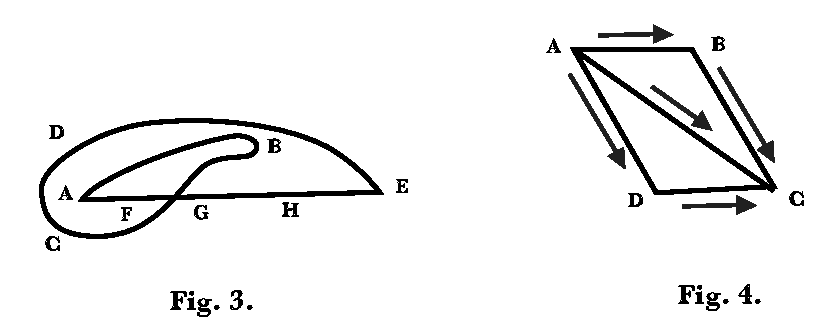
\includegraphics[width=3.6in]{peirce-howto2.pdf}

All this is purely conventional. It simply amounts to this: that we choose to call paths having the relations I have described equal or added. But, though it is a convention, it is a convention with a good reason. The rule for geometrical addition may be applied not only to paths, but to any other things which can be represented by paths. Now, as a path is determined by the varying direction and distance of the point which moves over it from the starting-point, it follows that anything which from its beginning to its end is determined by a varying direction and a varying magnitude is capable of being represented by a line. Accordingly, \emph{velocities} may be represented by lines, for they have only directions and rates. The same thing is true of \emph{accelerations,} or changes of velocities. This is evident enough in the case of velocities; and it becomes evident for accelerations if we consider that precisely what velocities are to positions--- namely, states of change of them--- that accelerations are to velocities.


The so-called ``parallelogram of forces'' is simply a rule for compounding accelerations. The rule is, to represent the accelerations by paths, and then to geometrically add the paths. The geometers, however, not only use the ``parallelogram of forces'' to compound different accelerations, but also to resolve one acceleration into a sum of several. Let \emph{A B} (Fig. 5) be the path which represents a certain acceleration--- say, such a change in the motion of a body that at the end of one second the body will, under the influence of that change, be in a position different from what it would have had if its motion had  continued unchanged such that a path equivalent to \emph{A B} would lead from the latter position to the former. This acceleration may be considered as the sum of the accelerations represented by \emph{A C} and \emph{C B.} It may also be considered as the sum of the very different accelerations represented by \emph{A D} and \emph{D B,} where \emph{A D} is almost the opposite of \emph{A C.} And it is clear that there is an immense variety of ways in which \emph{A B} might be resolved into the sum of two accelerations.

\centerline{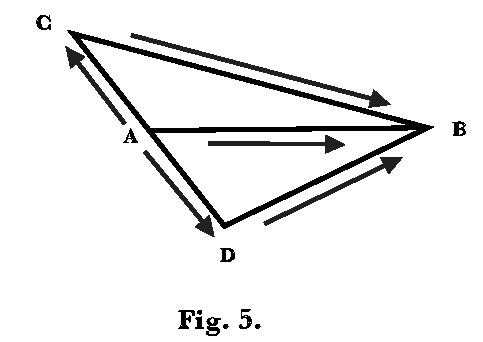
\includegraphics[width=1.6in]{peirce-howto3.pdf}}

After this tedious explanation, which I hope, in view of the extraordinary interest of the conception of force, may not have exhausted the reader's patience, we are prepared at last to state the grand fact which this conception embodies. This fact is that if the actual changes of motion which the different particles of bodies experience are each resolved in its appropriate way, each component acceleration is precisely such as is prescribed by a certain law of Nature, according to which bodies in the relative positions which the bodies in question actually have at the moment\authornote{Possibly the velocities also have to be taken into account.} always receive certain accelerations, which, being compounded by geometrical addition, give the acceleration which the body actually experiences.


This is the only fact which the idea of force represents, and whoever will take the trouble clearly to apprehend what this fact is, perfectly comprehends what force is. Whether we ought to say that a force \emph{is} an acceleration, or that it \emph{causes} an acceleration, is a mere question of propriety of language, which has no more to do with our real meaning than the difference between the French idiom ``\emph{Il fait froid}'' and its English equivalent ``\emph{It is cold}.'' Yet it is surprising to see how this simple affair has muddled men's minds. In how many profound treatises is not force spoken of as a ``mysterious entity,'' which seems to be only a way of confessing that the author despairs of ever getting a clear notion of what the word means! In a recent admired work on Analytic Mechanics it is stated that we understand precisely the effect of force, but what force itself is we do not understand! This is simply a self-contradiction. The idea which the word force excites in our minds has no other function than to affect our actions, and these actions can have no reference to force otherwise than through its effects. Consequently, if we know what the effects of force are, we are acquainted with every fact which is implied in saying that a force exists, and there is nothing more to know. The truth is, there is some vague notion afloat that a question may  mean something which the mind cannot conceive; and when some hair-splitting philosophers have been confronted with the absurdity of such a view, they have invented an empty distinction between positive and negative conceptions, in the attempt to give their non-idea a form not obviously nonsensical. The nullity of it is sufficiently plain from the considerations given a few pages back; and, apart from those considerations, the quibbling character of the distinction must have struck every mind accustomed to real thinking.

\subsection*{IV}



Let us now approach the subject of logic, and consider a conception which particularly concerns it, that of \emph{reality.} Taking clearness in the sense of familiarity, no idea could be clearer than this. Every child uses it with perfect confidence, never dreaming that he does not understand it. As for clearness in its second grade, however, it would probably puzzle most men, even among those of a reflective turn of mind, to give an abstract definition of the real. Yet such a definition may perhaps be reached by considering the points of difference between reality and its opposite, fiction. A figment is a product of somebody's imagination; it has such characters as his thought impresses upon it. That those characters are independent of how you or I think is an external reality. There are, however, phenomena within our own minds, dependent upon our thought, which are at the same time real in the sense that we really think them. But though their characters depend on how we think, they do not depend on what we think those characters to be. Thus, a dream has a real existence as a mental phenomenon, if somebody has really dreamt it; that he dreamt so and so, does not depend on what anybody thinks was dreamt, but is completely independent of all opinion on the subject. On the other hand, considering, not the fact of dreaming, but the thing dreamt, it retains its peculiarities by virtue of no other fact than that it was dreamt to possess them. Thus we may define the real as that whose characters are independent of what anybody may think them to be. 
 
But, however satisfactory such a definition may be found, it would be a great mistake to suppose that it makes the idea of reality perfectly clear. Here, then, let us apply our rules. According to them, reality, like every other quality, consists in the peculiar sensible effects which things partaking of it produce. The only effect which real things have is to cause belief, for all the sensations which they excite emerge into  consciousness in the form of beliefs. The question therefore is, how is true belief (or belief in the real) distinguished from false belief (or belief in fiction). Now, as we have seen in the former paper, the ideas of truth and falsehood, in their full development, appertain exclusively to the experiential method of settling opinion. A person who arbitrarily chooses the propositions which he will adopt can use the word truth only to emphasize the expression of his determination to hold on to his choice. Of course, the method of tenacity never prevailed exclusively; reason is too natural to men for that. But in the literature of the dark ages we find some fine examples of it. When Scotus Erigena is commenting upon a poetical passage in which hellebore is spoken of as having caused the death of Socrates, he does not
hesitate to inform the inquiring reader that Helleborus and Socrates were two eminent Greek philosophers, and that the latter, having been overcome in argument by the former, took the matter to heart and died of it! What sort of an idea of truth could a man have who could adopt and teach, without the qualification of a perhaps, an opinion taken so entirely at random? The real spirit of Socrates, who I hope would have been delighted to have been ``overcome in argument,'' because he would have learned something by it, is in curious contrast with the naive idea of the glossist, for whom discussion would seem to have been simply a struggle. When philosophy began to awake from its long slumber, and before theology completely dominated it, the practice seems to have been for each professor to seize upon any philosophical position he found unoccupied and which seemed a strong one, to intrench himself in it, and to sally forth from time to time to give battle to the others. Thus, even the scanty records we possess of those disputes enable us to make out a dozen or more opinions held by different teachers at one time concerning the question of nominalism and realism. Read the opening part of the ``Historia Calamitatum'' of Abelard, who was certainly as philosophical as any of his contemporaries, and see the spirit of
combat which it breathes. For him, the truth is simply his particular stronghold. When the method of authority prevailed, the truth meant little more than the Catholic faith. All the efforts of the scholastic doctors are directed toward harmonizing their faith in Aristotle and their faith in the Church, and one may search their ponderous folios through without finding an argument which goes any further. It is noticeable that where different faiths flourish side by side, renegades are looked upon with contempt even by the party whose belief they adopt; so completely has the idea of loyalty replaced that of truth-seeking. Since the  time of Descartes, the defect in the conception of truth has been less apparent. Still, it will sometimes strike a scientific man that the philosophers have been less intent on finding out what the facts are, than on inquiring what belief is most in harmony with their system. It is hard to convince a follower of the \emph{a priori} method by adducing facts; but show him that an opinion he is defending is inconsistent with what he has laid down elsewhere, and he will be very apt to retract it. These minds do not seem to believe that disputation is ever to cease; they seem to think that the opinion which is natural for one man is not so for another, and that belief will, consequently, never be settled. In contenting themselves with fixing their own opinions by a method which would lead another man to a different result, they betray their feeble hold of the conception of what truth is. 

On the other hand, all the followers of science are animated by a cheerful hope that the processes of investigation, if only pushed far enough, will give one certain solution to each question to which they can be applied. One man may investigate the velocity of light by studying the
transits of Venus and the aberration of the stars; another by the oppositions of Mars and the eclipses of Jupiter's satellites; a third by the method of Fizeau; a fourth by that of Foucault; a fifth by the motions of the curves of
Lissajoux; a sixth, a seventh, an eighth, and a ninth, may follow the different methods of comparing the measures of statical and dynamical electricity. They may at first obtain different results, but, as each perfects his method and his processes, the results are found to move steadily together toward a destined center. So with all scientific research. Different minds may set out with the most antagonistic views, but the progress of investigation carries them by a force outside of themselves to one and the same conclusion. This activity of thought by which we are carried, not where we wish, but to a fore-ordained goal, is like the operation of destiny. No modification of the
point of view taken, no selection of other facts for study, no natural bent of mind even, can enable a man to escape the predestinate opinion. This great law is embodied in the conception of truth and reality. The opinion which is fated\authornote{Fate means merely that which is sure to come true, and can nohow be avoided. It is a superstition to suppose that a certain sort of events are ever fated, and it is another to suppose that the word fate can never be freed from its superstitious taint. We are all fated to die.} to be ultimately agreed to by all who investigate, is what we mean by the truth, and the object represented in this opinion is the real. That is the way I would explain reality.


But it may be said that this view is directly opposed to the abstract  definition which we have given of reality, inasmuch as it makes the characters of the real depend on what is ultimately thought about them. But the answer to this is that, on the one hand, reality is independent, not necessarily of thought in general, but only of what you or I or any finite number of men may think about it; and that, on the other hand, though the
object of the final opinion depends on what that opinion is, yet what that opinion is does not depend on what you or I or any man thinks. Our perversity and that of others may indefinitely postpone the settlement of opinion; it
might even conceivably cause an arbitrary proposition to be universally accepted as long as the human race should last. Yet even that would not change the nature of the belief, which alone could be the result of investigation
carried sufficiently far; and if, after the extinction of our race, another should arise with faculties and disposition for investigation, that true opinion must be the one which they would ultimately come to. ``Truth crushed to
earth shall rise again,'' and the opinion which would finally result from investigation does not depend on how anybody may actually think. But the reality of that which is real does depend on the real fact that investigation
is destined to lead, at last, if continued long enough, to a belief in it. 



But I may be asked what I have to say to all the minute facts of history, forgotten never to be recovered, to the lost books of the ancients, to the buried secrets.
\begin{quote}
Full many a gem of purest ray serene\\
The dark, unfathomed caves of ocean bear;\\
Full many a flower is born to blush unseen,\\
And waste its sweetness on the desert air.
\end{quote}
Do these things not really exist because they are hopelessly beyond the reach of our knowledge? And then, after the universe is dead (according to the prediction of some scientists), and all life has ceased forever, will not the shock of atoms continue though there will be no mind to know it? To this I reply that, though in no possible state of knowledge can any number be great enough to express the relation between the amount of what rests unknown to the amount of the known, yet it is unphilosophical to suppose that, with regard to any given question (which has any clear meaning), investigation would not bring forth a solution of it, if it were carried far enough. Who would have said, a few years ago, that we could ever know of what substances stars are made whose light may have been longer in reaching us than the human race has existed? Who can be sure of  what we shall not know in a few hundred years? Who can guess what would be the result of continuing the pursuit of science for ten thousand years, with the activity of the last hundred? And if it were to go on for a million, or a billion, or any number of years you please, how is it possible to say that there is any question which might not ultimately be solved?


But it may be objected, ``Why make so much of these remote considerations, especially when it is your principle that only practical distinctions have a meaning?'' Well, I must confess that it makes very little difference whether we say that a stone on the bottom of the ocean, in complete darkness, is brilliant or not--- that is to say, that it
\emph{probably} makes no difference, remembering always that stone \emph{may} be fished up tomorrow. But that there are gems at the bottom of the sea, flowers in the untraveled desert, etc., are propositions which,  like that about a diamond being hard when it is not pressed, concern much more the arrangement of our language than they do the meaning of our ideas. 

It seems to me, however, that we have, by the
application of our rule, reached so clear an apprehension of what we mean by reality, and of the fact which the idea rests on, that we should not, perhaps, be making a pretension so presumptuous as it would be singular, if we were to
offer a metaphysical theory of existence for universal acceptance among those who employ the scientific method of fixing belief. However, as metaphysics is a subject much more curious than useful, the knowledge of which, like that of a sunken reef, serves chiefly to enable us to keep clear of it, I will not trouble the reader with any more Ontology at this moment. I have already been led much further into that path than I should have desired; and I have given the reader such a dose of mathematics, psychology, and all that is most abstruse, that I fear he may already have left me, and that what I am now writing is for the compositor and proof-reader exclusively. I trusted to the
importance of the subject. There is no royal road to logic, and really valuable ideas can only be had at the price of close attention. But I know that in the matter of ideas the public prefer the cheap and nasty; and in my next paper I am going to return to the easily intelligible, and not wander from it again. The reader who has been at the pains of wading through this paper, shall be rewarded in the next one by seeing how beautifully what has been developed in this tedious way can be applied to the ascertainment of the rules of scientific reasoning.


We have, hitherto, not crossed the threshold of scientific logic. It  is certainly important to know how to make our ideas clear, but they may be ever so clear without being true. How to make them so, we have next to study. How to give birth to those vital and procreative ideas which multiply into a thousand forms and diffuse themselves everywhere, advancing civilization and making the dignity of man, is an art not yet reduced to rules, but of the secret of which the history of science affords some hints.



% This file does not have the appropriate header and tags to compile in latex. It is meant to be input into another file for compiling. 



\section*{The Doctrine of Chances}
\emph{This is part three in the series. It was originally published in \emph{Popular Science Monthly} 12 (March 1878), pgs. 604--615.}

\subsection*{I}

It is a common observation that a science first begins to be exact when it is quantitatively treated. What are called the exact sciences are no others than the mathematical ones. Chemists reasoned vaguely until Lavoisier showed them how to apply the balance to the verification of their theories, when chemistry leaped suddenly into the position of the most perfect of the classificatory sciences. It has thus become so precise and certain that we usually think of it along with optics, thermotics, and electrics. But these are studies of general laws, while chemistry considers merely the relations and classification of certain objects; and belongs, in reality, in the same category as systematic botany and zo\"ology. Compare it with these last, however, and the advantage that it derives from its quantitative treatment is very evident.

The rudest numerical scales, such as that by which the mineralogists distinguish the different degrees of hardness, are found useful. The mere counting of pistils and stamens sufficed to bring botany out of total chaos into some hind of form. It is not, however, so much from \emph{counting} as from \emph{measuring}, not so much from the conception of number as from that of continuous quantity, that the advantage of mathematical treatment comes. Number, after all, only serves to pin us down to a precision in our thoughts which, however beneficial, can seldom lead to lofty conceptions, and frequently descends to pettiness. Of those two faculties of which Bacon speaks, that which marks differences and that which notes resemblances, the employment of number can only aid the lesser one; and the excessive use of it must tend to narrow the powers of the mind. But the conception of continuous quantity has a great office to fulfill, independently of any attempt at precision. Far from tending to the exaggeration of differences, it is the direct instrument of the finest generalizations. When a naturalist wishes to study a species, he collects a considerable number of specimens more or less similar. In contemplating them, he observes certain ones which are more or less alike in some particular respect. They all have, for instance, a certain S-shaped marking. He observes that they are not \emph{precisely} alike, in this respect; the S has not precisely the same shape, but the differences are such as to lead him to believe that forms could be found intermediate between any two of those he possesses. He, now, finds other forms apparently quite dissimilar--- say a marking in the form of a C--- and the question is, whether he can find intermediate ones which will connect these latter with the others. This he often succeeds in doing in cases where it would at first be thought impossible; whereas, he sometimes finds those which differ, at first glance, much less, to be separated in Nature by the non-occurrence of intermediaries. In this way, he builds up from the study of Nature a new general conception of the character in question. He obtains, for example, an idea of a leaf which includes every part of the flower, and an idea of a vertebra which includes the skull. I surely need not say much to show what a logical engine there is here. It is the essence of the method of the naturalist. How he applies it first to one character, and then to another, and finally obtains a notion of a species of animals, the differences between whose members, however great, are confined within limits, is a matter which does not here concern us. The whole method of classification must be considered later; but, at present, I only desire to point out that it is by taking advantage of the idea of continuity, or the passage from one form to another by insensible degrees, that the naturalist builds his conceptions. Now, the naturalists are the great builders of conceptions; there is no other branch of science where so much of this work is done as in theirs; and we must, in great measure, take them for our teachers in this important part of logic. And it will be found everywhere that the idea of continuity is a powerful aid to the formation of true and fruitful conceptions. By means of it, the greatest differences are broken down and resolved into differences of degree, and the incessant application of it is of the greatest value in broadening our conceptions. I propose to make a great use of this idea in the present series of papers; and the particular series of important fallacies, which, arising from a neglect of it, have desolated philosophy, must further on be closely studied. At present, I simply call the reader's attention to the utility of this conception.

In studies of numbers, the idea of continuity is so indispensable, that it is perpetually introduced even where there is no continuity in fact, as where we say that there are in the United States 10.7 inhabitants per square mile, or that in New York 14.72 persons live in the average house.\footnote{This mode of thought is so familiarly associated with all exact numerical consideration, that the phrase appropriate to it is imitated by shallow writers in order to produce of the appearance of exactitude where none exists. Certain newspapers which affect a learned tone talk of ``the average man,'' when they simply mean \emph{most men}, and have no idea of striking an average.} Another example is that law of the distribution of errors which Quetelet, Galton, and others, have applied with so much success to the study of biological and social matters. This application of continuity to cases where it does not really exist illustrates, also, another point which will hereafter demand a separate study, namely, the great utility which fictions sometimes have in science.

\subsection*{II}

The theory of probabilities is simply the science of logic quantitatively treated. There are two conceivable certainties with reference to any hypothesis, the certainty of its truth and the certainty of its falsity. The numbers \emph{one} and \emph{zero} are appropriated, in this calculus, to marking these extremes of knowledge; while fractions having values intermediate between them indicate, as we may vaguely say, the degrees in which the evidence leans toward one or the other. The general problem of probabilities is, from a given state of facts, to determine the numerical probability of a possible fact. This is the same as to inquire how much the given facts are worth, considered as evidence to prove the possible fact. Thus the problem of probabilities is simply the general problem of logic.

Probability is a continuous quantity, so that great advantages may be expected from this mode of studying logic. Some writers have gone so far as to maintain that, by means of the calculus of chances, every solid inference may be represented by legitimate arithmetical operations upon the numbers given in the premises. If this be, indeed, true, the great problem of logic, how it is that the observation of one fact can give us knowledge of another independent fact, is reduced to a mere question of arithmetic. It seems proper to examine this pretension before undertaking any more recondite solution of the paradox.

But, unfortunately, writers on probabilities are not agreed in regard to this result. This branch of mathematics is the only one, I believe, in which good writers frequently get results entirely erroneous. In elementary geometry the reasoning is frequently fallacious, but erroneous conclusions are avoided; but it may be doubted if there is a single extensive treatise on probabilities in existence which does not contain solutions absolutely indefensible. This is partly owing to the want of any regular method of procedure; for the subject involves too many subtilties to make it easy to put its problems into equations without such an aid. But, beyond this, the fundamental principles of its calculus are more or less in dispute. In regard to that class of questions to which it is chiefly applied for practical purposes, there is comparatively little doubt; but in regard to others to which it has been sought to extend it, opinion is somewhat unsettled.

This last class of difficulties can only be entirely overcome by making the idea of probability perfectly clear in our minds in the way set forth in our last paper.

\subsection*{III}

To get a clear idea of what we mean by probability, we have to consider what real and sensible difference there is between one degree of probability and another.

The character of probability belongs primarily, without doubt, to certain inferences. Locke explains it as follows: After remarking that the mathematician positively knows that the sum of the three angles of a triangle is equal to two right angles because he apprehends the geometrical proof, he thus continues: \begin{quote}
But another man who never took the pains to observe the demonstration, hearing a mathematician, a man of credit, affirm the three angles of a triangle to be equal to two right ones,\emph{assents} to it; i.e., receives it for true. In which case the foundation of his assent is the probability of the thing, the proof being such as, for the most part, carries truth with it; the man on whose testimony he receives it not being wont to affirm anything contrary to, or besides his knowledge, especially in matters of this kind.
\end{quote}
The celebrated \emph{Essay concerning Humane Understanding} contains many passages which, like this one, make the first steps in profound analyses which are not further developed. It was shown in the first of these papers that the validity of an inference does not depend on any tendency of the mind to accept it, however strong such tendency may be; but consists in the real fact that, when premises like those of the argument in question are true, conclusions related to them like that of this argument are also true. It was remarked that in a logical mind an argument is always conceived as a member of a genus of arguments all constructed in the same way, and such that, when their premises are real facts, their conclusions are so also. If the argument is demonstrative, then this is always so; if it is only probable, then it is for the most part so. As Locke says, the probable argument is ``\emph{such as} for the most part carries truth with it.''

According to this, that real and sensible difference between one degree of probability and another, in which the meaning of the distinction lies, is that in the frequent employment of two different modes of inference, one will carry truth with it oftener than the other. It is evident that this is the only difference there is in the existing fact. Having certain premises, a man draws a certain conclusion, and as far as this inference alone is concerned the only possible practical question is whether that conclusion is true or not, and between existence and non-existence there is no middle term. ``Being only is and nothing is altogether not,'' said Parmenides; and this is in strict accordance with the analysis of the conception of reality given in the last paper. For we found that the distinction of reality and fiction depends on the supposition that sufficient investigation would cause one opinion to he universally received and all others to he rejected. That presupposition involved in the very conceptions of reality and figment involves a complete sundering of the two. It is the heaven-and-hell idea in the domain of thought. But, in the long run, there is a real fact which corresponds to the idea of probability, and it is that a given mode of inference sometimes proves successful and sometimes not, and that in a ratio ultimately fixed. As we go on drawing inference after inference of the given kind, during the first ten or hundred cases the ratio of successes may he expected to show considerable fluctuations; but when we come into the thousands and millions, these fluctuations become less and less; and if we continue long enough, the ratio will approximate toward a fixed limit. We may therefore define the probability of a mode of argument as the proportion of cases in which it carries truth with it.

The inference from the premise, A, to the conclusion, B, depends, as we have seen, on the guiding principle, that if a fact of the class A is true, a fact of the class B is true. The probability consists of the fraction whose numerator is the number of times in which both A and B are true, and whose denominator is the total number of times in which A is true, whether B is so or not. Instead of speaking of this as the probability of the inference, there is not the slighest objection to calling it the probability that, if A happens, B happens. But to speak of the probability of the event B, without naming the condition, really has no meaning at all. It is true that when it is perfectly obvious what condition is meant, the ellipsis may be permitted. But we should avoid contracting the habit of using language in this way (universal as the habit is), because it gives rise to a vague way of thinking, as if the action of causation might either determine an event to happen or determine it not to happen, or leave it more or less free to happen or not, so as to give rise to an \emph{inherent} chance in regard to its occurrence. It is quite clear to me that some of the worst and most persistent errors in the use of the doctrine of chances have arisen from this vicious mode of expression.\footnote{The conception of probability here set forth is substantially that first developed by Mr. Venn, in his ``Logic of Chance.'' Of course, a vague apprehension of the idea had always existed, but the problem was to make it perfectly clear, and to him belongs the credit of first doing this.}

\subsection*{IV}


But there remains an important point to he cleared up. According to what has been said, the idea of probability essentially belongs to a kind of inference which is repeated indefinitely. An individual inference must be either true or false, and can show no effect of probability; and, therefore, in reference to a single case considered in itself, probability can have no meaning. Yet if a man bad to choose between drawing a card from a pack containing twenty-five red cards and a black one, or from a pack containing twenty-five black cards and a red one, and if the drawing of a red card were destined to transport him to eternal felicity, and that of a black one to consign him to everlasting woe, it would be folly to deny that he ought to prefer the pack containing the larger proportion of red cards, although, from the nature of the risk, it could not be repeated. It is not easy to reconcile this with our analysis of the conception of chance. But suppose he should choose the red pack, and should draw the wrong card, what consolation would he have? He might say that he had acted in accordance with reason, but that would only show that his reason was absolutely worthless. And if he should choose the right card, how could he regard it as anything but a happy accident? He could not say that if he had drawn from the other pack, he might have drawn the wrong one, because an hypothetical proposition such as, ``if A, then B,'' means nothing with reference to a single case. Truth consists in the existence of a real fact corresponding to the true proposition. Corresponding to the proposition, ``if A, then B,'' there may be the fact that \emph{whenever} such an event as A happens such an event as B happens. But in the case supposed, which has no parallel as far as this man is concerned, there would be no real fact whose existence could give any truth to the statement that, if he had drawn from the other pack, he might have drawn a black card. Indeed, since the validity of an inference consists in the truth of the hypothetical proposition that \emph{if} the premises be true the conclusion will also be true, and since the only real fact which can correspond to such a proposition is that whenever the antecedent is true the consequent is so also, it follows that there can be no sense in reasoning in an isolated case, at all.

These considerations appear, at first sight, to dispose of the difficulty mentioned. Yet the case of the other side is not yet exhausted. Although probability will probably manifest its effect in, say, a thousand risks, by a certain proportion between the numbers of successes and failures, yet this, as we have seen, is only to say that it certainly will, at length, do so. Now the number of risks, the number of probable inferences, which a man draws in his whole life, is a finite one, and he cannot be absolutely \emph{certain} that the mean result will accord with the probabilities at all. Taking all his risks collectively, then, it cannot be certain that they will not fail, and his case does not differ, except in degree, from the one last supposed. It is an indubitable result of the theory of probabilities that every gambler, if he continues long enough, must ultimately be ruined. Suppose he tries the martingale, which some believe infallible, and which is, as I am informed, disallowed in the gambling-houses. In this method of playing, he first bets say \$1; if he loses it he bets \$2; if he loses that he bets \$4; if he loses that he bets \$8; if he then gains he has lost $1+2+4=7$, and he has gained \$1 more; and no matter how many bets he loses, the first one he gains will make him \$1 richer than he was in the beginning. In that way, he will probably gain at first; but, at last, the time will come when the run of luck is so against him that he will not have money enough to double, and must therefore let his bet go. This will \emph{probably} happen before he has won as much as he had in the first place, so that this run against him will leave him poorer than he began; some time or other it will be sure to happen. It is true that there is always a possibility of his winning any sum the bank can pay, and we thus come upon a celebrated paradox that, though he is certain to be ruined, the value of his expectation calculated according to the usual rules (which omit this consideration) is large. But, whether a gambler plays in this way or any other, the same thing is true, namely, that if plays long enough he will be sure some time to have such a run against him as to exhaust his entire fortune. The same thing is true of an insurance company. Let the directors take the utmost pains to be independent of great conflagrations and pestilences, their actuaries can tell them that, according to the doctrine of chances, the time must come, at last, when their losses will bring them to a stop. They may tide over such a crisis by extraordinary means, but then they will start again in a weakened state, and the same thing will happen again all the sooner. An actuary might be inclined to deny this, because he knows that the expectation of his company is large, or perhaps (neglecting the interest upon money) is infinite. But calculations of expectations leave out of account the circumstance now under consideration, which reverses the whole thing. However, I must not be understood as saying that insurance is on this account unsound, more than other kinds of business. All human affairs rest upon probabilities, and the same thing is true everywhere. If man were immortal he could be perfectly sure of seeing the day when everything in which he had trusted should betray his trust, and, in short, of coming eventually to hopeless misery. He would break down, at last, as every great fortune, as every dynasty, as every civilization does. In place of this we have death.

But what, without death, would happen to every man, with death must happen to some man. At the same time, death makes the number of our risks, of our inferences, finite, and so makes their mean result uncertain. The very idea of probability and of reasoning rests on the assumption that this number is indefinitely great. We are thus landed in the same difficulty as before, and I can see but one solution of it. It seems to me that we are driven to this, that logicality inexorably requires that our interests shall \emph{not} be limited. They must not stop at our own fate, but must embrace the whole community. This community, again, must not be limited, but must extend to all races of beings with whom we can come into immediate or mediate intellectual relation. It must reach, however vaguely, beyond this geological epoch, beyond all bounds. He who would not sacrifice his own soul to save the whole world, is, as it seems to me, illogical in all his inferences, collectively. Logic is rooted in the social principle.

To be logical men should not be selfish; and, in point of fact, they are not so selfish as they are thought. The willful prosecution of one's desires is a different thing from selfishness. The miser is not selfish; his money does him no good, and he cares for what shall become of it after his death. We are constantly speaking of \emph{our} possessions on the Pacific, and of \emph{our} destiny as a republic, where no personal interests are involved, in a way which shows that we have wider ones. We discuss with anxiety the possible exhaustion of coal in some hundreds of years, or the cooling-off of the sun in some millions, and show in the most popular of all religious tenets that we can conceive the possibility of a man's descending into hell for the salvation of his fellows.

Now, it is not necessary for logicality that a man should himself be capable of the heroism of self-sacrifice. It is sufficient that he should recognize the possibility of it, should perceive that only that man's inferences who has it are really logical, and should consequently regard his own as being only so far valid as they would be accepted by the hero. So far as he thus refers his inferences to that standard, he becomes identified with such a mind.

This makes logicality attainable enough. Sometimes we can personally attain to heroism. The soldier who runs to scale a wall knows that he will probably be shot, but that is not all he cares for. He also knows that if all the regiment, with whom in feeling he identifies himself, rush forward at once, the fort will be taken. In other cases we can only imitate the virtue. The man whom we have supposed as having to draw from the two packs, who if he is not a logician will draw from the red pack from mere habit, will see, if he is logician enough, that he cannot be logical so long as he is concerned only with his own fate, but that that man who should care equally for what was to happen in all possible cases of the sort could act logically, and would draw from the pack with the most red cards, and thus, though incapable himself of such sublimity, our logician would imitate the effect of that man's courage in order to share his logicality.

But all this requires a conceived identification of one's interests with those of an unlimited community. Now, there exist no reasons, and a later discussion will show that there can be no reasons, for thinking that the human race, or any intellectual race, will exist forever. On the other hand, there can be no reason against it;\footnote{I do not here admit an absolutely unknowable. Evidence could show us what would probably be the case after any given lapse of time; and though a subsequent time might be assigned which that evidence might not cover, yet further evidence would cover it.} and, fortunately, as the whole requirement is that we should have certain sentiments, there is nothing in the facts to forbid our having a hope, or calm and cheerful wish, that the community may last beyond any assignable date.

It may seem strange that I should put forward three sentiments, namely, interest in an indefinite community, recognition of the possibility of this interest being made supreme, and hope in the unlimited continuance of intellectual activity, as indispensable requirements of logic. Yet, when we consider that logic depends on a mere struggle to escape doubt, which, as it terminates in action, must begin in emotion, and that, furthermore, the only cause of our planting ourselves on reason is that other methods of escaping doubt fail on account of the social impulse, why should we wonder to find social sentiment presupposed in reasoning? As for the other two sentiments which I find necessary, they are so only as supports and accessories of that. It interests me to notice that these three sentiments seem to be pretty much the same as that famous trio of Charity, Faith, and Hope, which, in the estimation of St. Paul, are the finest and greatest of spiritual gifts. Neither Old nor New Testament is a text-book of the logic of science, but the latter is certainly the highest existing authority in regard to the dispositions of heart which a man ought to have.

\subsection*{V}

Such average statistical numbers as the number of inhabitants per square mile, the average number of deaths per week, the number of convictions per indictment, or, generally speaking, the number of x's per y, where the x's are a class of things some or all of which are connected with another class of things, their y's, I term \emph{relative} numbers. Of the two classes of things to which a relative number refers, that one of which it is a number may be called its \emph{relate}, and that one per which the numeration is made may be called its \emph{correlate}.

Probability is a kind of relative number; namely, it is the ratio of the number of arguments of a certain genus which carry truth with them to the total number of arguments of that genus, and the rules for the calculation of probabilities are very easily derived from this consideration. They may all be given here, since they are extremely simple, and it is sometimes convenient to know something of the elementary rules of calculation of chances.

\paragraph{Rule I. Direct Calculation.} --- To calculate, directly, any relative number, say for instance the number of passengers in the average trip of a street-car, we must proceed as follows:

Count the number of passengers for each trip; add all these numbers, and divide by the number of trips. There are cases in which this rule may be simplified. Suppose we wish to know the number of inhabitants to a dwelling in New York. The same person cannot inhabit two dwellings. If he divide his time between two dwellings he ought to be counted a half-inhabitant of each. In this case we have only to divide the total number of the inhabitants of New York by the number of their dwellings, without the necessity of counting separately those which inhabit each one. A similar proceeding will apply wherever each individual relate belongs to one individual correlate exclusively. If we want the number of x's per y, and no x belongs to more than one y, we have only to divide the whole number of x's of y's by the number of y's. Such a method would, of course, fail if applied to finding the average number of street-car passengers per trip. We could not divide the total number of travelers by the number of trips, since many of them would have made many passages. To find the probability that from a given class of premises, A, a given class of conclusions, B, follow, it is simply necessary to ascertain what proportion of the times in which premises of that class are true, the appropriate conclusions are also true. In other words, it is the number of cases of the occurrence of both the events A and B, divided by the total number of cases of the occurrence of the event A.

\paragraph{Rule II. Addition of Relative Numbers.} --- Given two relative numbers having the same correlate, say the number of x's per y, and the number of z's per y; it is required to find the number of x's and z's together per y. If there is nothing which is at once an x and a z to the same y, the sum of the two given numbers would give the required number. Suppose, for example, that we had given the average number of friends that men have, and the average number of enemies, the sum of these two is the average number of persons interested in a man. On the other hand, it plainly would not do to add the average number of persons having constitutional diseases to the average number over military age, and to the average number exempted by each special cause from military service, in order to get the average number exempt in any way, since many are exempt in two or more ways at once.

This rule applies directly to probabilities. Given the probability that two different and mutually exclusive events will happen under the same supposed set of circumstances. Given, for instance, the probability that if A then B, and also the probability that if A then C, then the sum of these two probabilities is the probability that if A then either B or C, so long as there is no event which belongs at once to the two classes B and C.

\paragraph{Rule III. Multiplication of Relative Numbers.} --- Suppose that we have given the relative number of x's per y also the relative number of z's per x of y; or, to take a concrete example, suppose that we have given, first, the average number of children in families living in New York; and, second, the average number of teeth in the head of a New York child--- then the product of these two numbers would give the average number of children's teeth in a New York family. But this mode of reckoning will only apply in general under two restrictions. In the first place, it would not be true if the same child could belong to different families, for in that case those children who belonged to several different families might have an exceptionally large or small number of teeth, which would affect the average number of children's teeth in a family more than it would affect the average number of teeth in a child's head. In the second place, the rule would not be true if different children could share the same teeth, the average number of children's teeth being in that case evidently something different from the average number of teeth belonging to a child.

In order to apply this rule to probabilities, we must proceed as follows: Suppose that we have given the probability that the conclusion B follows from the premise A, B and A representing as usual certain classes of propositions. Suppose that we also knew the probability of an inference in which B should be the premise, and a proposition of a third kind, C, the conclusion. Here, then, we have the materials for the application of this rule. We have, first, the relative number of B's per A. We next should have the relative number of C's per B following from A. But the classes of propositions being so selected that the probability of C following from any B in general is just the same as the probability of C's following from one of those B's which is deducible from an A, the two probabilities may be multiplied together, in order to give the probability of C following from A. The same restrictions exist as before. It might happen that the probability that B follows from A was affected by certain propositions of the class B following from several different propositions of the class A. But, practically speaking, all these restrictions are of very little consequence, and it is usually recognized as a principle universally true that the probability that, if A is true, B is, multiplied by the probability that, if B is true, C is, gives the probability that, if A is true, C is.

There is a rule supplementary to this, of which great use is made. It is not universally valid, and the greatest caution has to be exercised in making use of it--- a double care, first, never to use it when it will involve serious error; and, second, never to fail to take advantage of it in cases in which it can be employed. This rule depends upon the fact that in very many cases the probability that C is true if B is, is substantially the same as the probability that C is true if A is. Suppose, for example, we have the average number of males among the children born in New York; suppose that we also have the average number of children born in the winter months among those born in New York. Now, we may assume without doubt, at least as a closely approximate proposition (and no very nice calculation would be in place in regard to probabilities), that the proportion of males among all the children born in New York is the same as the proportion of males born in summer in New York, and, therefore, if the names of all the children born during a year were put into an urn, we might multiply the probability that any name drawn would be the name of a male child by the probability that it would be the name of a child born in summer, in order to obtain the probability that it would be the name of a male child born in summer. The questions of probability, in the treatises upon the subject, have usually been such as relate to balls drawn from urns, and games of cards, and so on, in which the question of the \emph{independence} of events, as it is called--- that is to say, the question of whether the probability of C, under the hypothesis B, is the same as its probability under the hypothesis A, has been very simple; but, in the application of probabilities to the ordinary questions of life, it is often an exceedingly nice question whether two events may be considered as independent with sufficient accuracy or not. In all calculations about cards it is assumed that the cards are thoroughly shuffled, which makes one deal quite independent of another. In point of fact the cards seldom are, in practice, shuffled sufficiently to make this true; thus, in a game of whist, in which the cards have fallen in suits of four of the same suit, and are so gathered up, they will lie more or less in sets of four of the same suit, and this will be true even after they are shuffled. At least some traces of this arrangement will remain, in consequence of which the number of ``short suits,'' as they are called--- that is to say, the number of hands in which the cards are very unequally divided in regard to suits--- is smaller than the calculation would make it to be; so that, when there is a misdeal, where the cards, being thrown about the table, get very thoroughly shuffled, it is a common saying that in the hands next dealt out there are generally short suits. A few years ago a friend of mine, who plays whist a great deal, was so good as to count the number of spades dealt to him in 165 hands, in which the cards had been, if anything, shuffled better than usual. According to calculation, there should have been 85 of these hands in which my friend held either three or four spades, but in point of fact there were 94, showing the influence of imperfect shuffling.

According to the view here taken, these are the only fundamental rules for the calculation of chances. An additional one, derived from a different conception of probability, is given in some treatises, which if it be sound might be made the basis of a theory of reasoning. Being, as I believe it is, absolutely absurd, the consideration of it serves to bring us to the true theory; and it is for the sake of this discussion, which must be postponed to the next number, that I have brought the doctrine of chances to the reader's attention at this early stage of our studies of the logic of science.



\end{document} 